\section{Rate loss channels}
\label{subsec:rate-loss-channels}

The ions are stored up to a maximum of 6 seconds, often this leads to a trap loss of stored ions \cite{mikosch_evaporation_2007, mikosch_evaporation_2008}. To include this loss channel, Eq. \ref{eqn:rate:parent-ion}, \ref{eqn:rate:n-1thcomplexes} and \ref{eqn:rate:nth-complexes} are modified into the following:

\begin{equation}
    \frac{d\cd^+}{dt} = \text{Eq. } \ref{eqn:rate:parent-ion} - R_{loss} \cdot \cd^+
    \label{eqn:rate:modified:parent-ion}
\end{equation}

\begin{equation}
    \frac{d\text{He}_{n-1}\cd^+}{dt} = \text{Eq. } \ref{eqn:rate:n-1thcomplexes} - R_{loss} \cdot \text{He}_{n-1}\cd^+
    \label{eqn:rate:modified:n-1complexes}
\end{equation}

\begin{equation}
    \frac{d\text{He}_{n}\cd^+}{dt} = \text{Eq. } \ref{eqn:rate:nth-complexes} - R_{loss} \cdot \text{He}_{n}\cd^+
    \label{eqn:rate:modified:nth-complexes}
\end{equation}

where $R_{loss}$ indicates the trap loss rate [in \pers] . In addition to the
$R_{loss}$ channel, we have noticed a growth of m/z=30, which has been seen
even at a very low pressure where no higher order complexes are formed except He\CD, as
shown in Figure \ref{fig:trap-and-m30-loss-channel-comparision}. Therefore,
this channel is accounted for by adding an additional loss channel, as shown
below:

\begin{equation}
    \frac{d\cd^+}{dt} = \text{Eq. } \ref{eqn:rate:modified:parent-ion} - R_{loss30} \cdot \cd^+
    \label{eqn:rate:parent-ion-mass30-loss}
\end{equation}

The most probable candidate for m/z 30 is DCO$^+$, which could potentially form
at low temperatures by the following reaction with CO$_2$ or H$_2$O neutrals
(as shown for the main CH$^+$ isotope in the KIDA database \cite{wakelam_2014_2015}):

\begin{equation}
    \cd^+ + \text{CO}_2 \xrightarrow{} \text{CO} + \text{DCO}^+
    \label{eqn:mass-30-reaction-with-CO2}
\end{equation}
\begin{equation}
    \cd^+ + \text{H$_2$O} \xrightarrow{} \text{H$_2$} + \text{DCO}^+
    \label{eqn:mass-30-reaction-with-water}
\end{equation}

\begin{equation}
    \frac{d\text{DCO}^+}{dt} = R_{loss30} \cdot \cd^+
    \label{eqn:rate:mass-30-formation}
\end{equation}

\begin{figure}[!htb]

    \centering

    \begin{subfigure}[b]{0.49\textwidth}
        \centering
        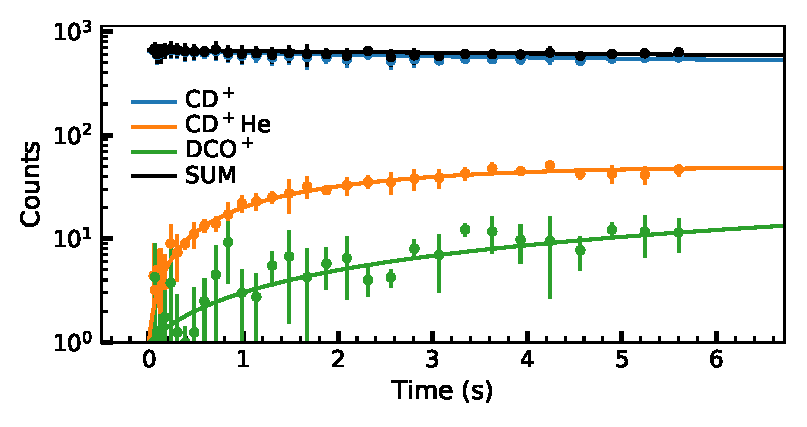
\includegraphics[width=1\textwidth]{figures/measurements/kinetics/loss_channels/m_30_loss_only.pdf}
        \caption{}
        
    \end{subfigure}
    \hfill
    \begin{subfigure}[b]{0.49\textwidth}
        \centering
        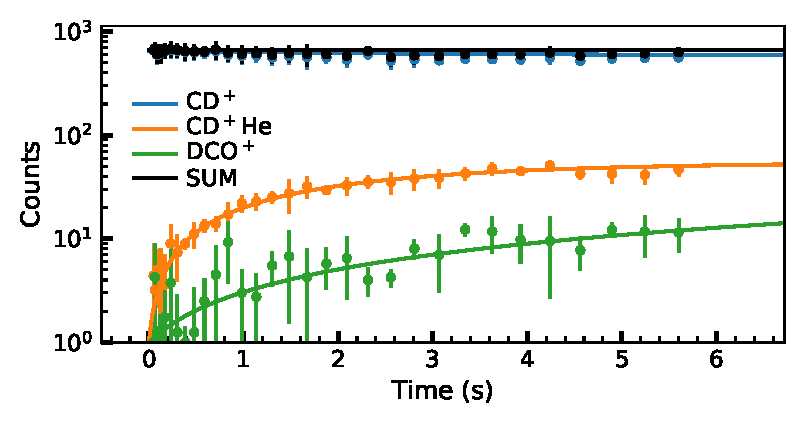
\includegraphics[width=1\textwidth]{figures/measurements/kinetics/loss_channels/trap_and_m_30_loss.pdf}
        % \includegraphics[width=1\textwidth]{figures/measurements/kinetics/compare-loss-channels-additions/without trap loss.pdf}
        \caption{}
        
    \end{subfigure}
    
    \begin{subfigure}[b]{0.49\textwidth}
        \centering
        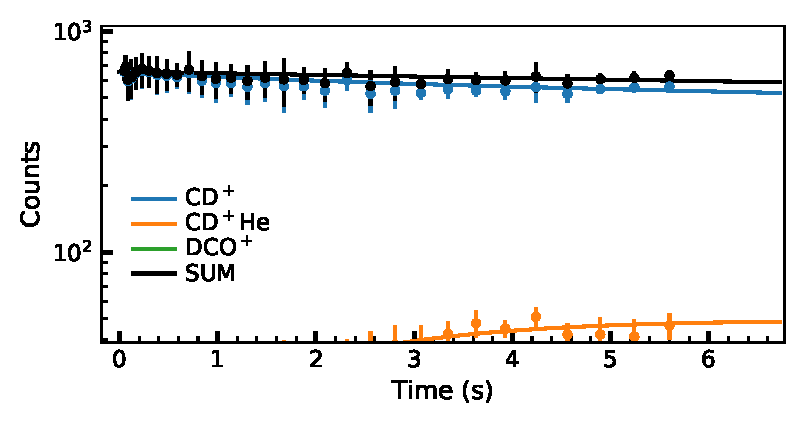
\includegraphics[width=1\textwidth]{figures/measurements/kinetics/loss_channels/m_30_loss_only_zoomed.pdf}
        \caption{}
        
    \end{subfigure}
    \hfill
    \begin{subfigure}[b]{0.49\textwidth}
        \centering
        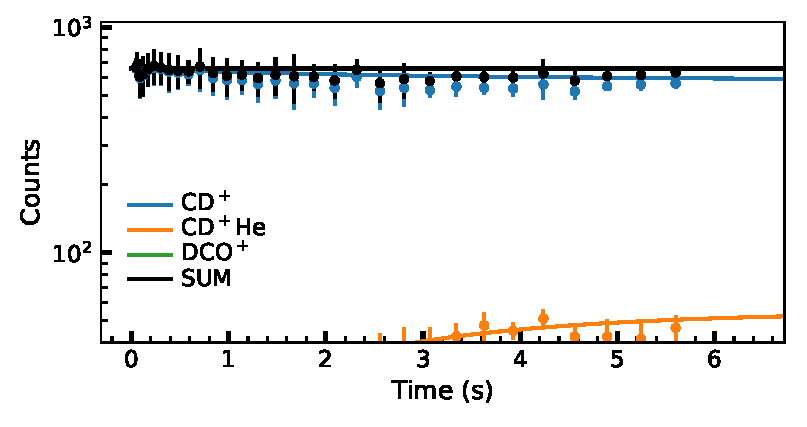
\includegraphics[width=1\textwidth]{figures/measurements/kinetics/loss_channels/trap_and_m_30_loss_zoomed.pdf}
        \caption{}
        
    \end{subfigure}
    
    % \begin{subfigure}[b]{0.49\textwidth}
    %     \centering
    %     \includegraphics[width=1\textwidth]{figures/measurements/kinetics/compare-loss-channels-additions/only mass 30[u] loss.pdf}
    %     \caption{}
    % \end{subfigure}
    
    % \hfill
    % \begin{subfigure}[b]{0.6\textwidth}
    %     \centering
    %     \includegraphics[width=1\textwidth]{figures/measurements/kinetics/compare-loss-channels-additions/trap + mass 30[u] loss.pdf}
    %     \caption{}
        
    % \end{subfigure}
    
    \caption{Fitting of the experimental kinetics scans to the rate equation model: (a) is with both $R_{loss}$ and $R_{loss30}$ channels included while (b) is only with $R_{loss30}$. (c) and (d) are zoomed-in regions for (a) and (b), respectively. The measurements were carried out at 6.9(3) K and  $1.770(45) \cdot 10^{14}$ \percc\ helium number density. No higher order complexes were formed other than mass 30, which most probably could be DCO$^+$ as described in Eq. \ref{eqn:mass-30-reaction-with-CO2} and \ref{eqn:mass-30-reaction-with-water}}
    
    % \caption{Comparing loss channels additions: (a) is with both $R_{loss}$ and $R_{loss30}$ channels included and no higher order complexes were formed other than mass 30 which most probably could be DCO$^+$ as described in Eq. \ref{eqn:mass-30-reaction-with-CO2} and \ref{eqn:mass-30-reaction-with-water}. The measurement for (a) were carried out at 6.9(3) K and  $1.770(45) \cdot 10^{14}$ \percc helium number density. To compare the effect of including extra trap loss channel, $R_{loss30}$  (b) and (c) are shown, without and with trap loss channel respectively measured at 4.8(3) K and $6.04(25) \cdot 10^{14}$ \percc number density.}
    \label{fig:trap-and-m30-loss-channel-comparision}
\end{figure}

Since the m/z 30 also corresponds to the He$_4$\CD complex, Eq.
\ref{eqn:rate:modified:n-1complexes} is modified only when $n-1=4$ (or Eq.
\ref{eqn:rate:modified:nth-complexes} when $n=4$) by adding the corresponding
loss channel \(R_{loss30} \cdot \cd^+\) as shown below:

\begin{equation}
    \frac{d(\text{He}_4\cd^+ + \text{DCO}^+)}{dt} = (\text{Eq. } \ref{eqn:rate:modified:n-1complexes} \text{ or } \ref{eqn:rate:modified:nth-complexes}) + R_{loss30} \cdot \cd^+
    \label{eqn:rate:mass-30-correction}
\end{equation}

The coupled ordinary differential equations for the parent ion \CD (Eq.
\ref{eqn:rate:parent-ion}, \ref{eqn:rate:modified:parent-ion} or
\ref{eqn:rate:parent-ion-mass30-loss}) and the formed complexes (Eq.
\ref{eqn:rate:n-1thcomplexes}, \ref{eqn:rate:nth-complexes} or
\ref{eqn:rate:mass-30-correction}) are used to numerically simulate and fit the
experimentally observed data to determine the rate constants, which is
discussed in more detail in the next section in different aspects. This complex formation 
process is vital for understanding the ROSAA spectroscopic technique employed in this work.
